\header{
    \section{Le duc de Bordeaux} \label{le-duc-de-bordeaux}
    %
    
    \insertComment{Réécriture faite par les 4 barbus en 1997.}{}
}

\enluminure{4}{\href{https://www.youtube.com/watch?v=3jqugzbZk18}{L}}{e duc} de Bordeaux ressemble à son père,
\\Son père qui était un illustre boxeur
\\Il en a gardé certaines manières
\\Qui choquent beaucoup tous les autres seigneurs.
\\\\Il essuie ses pieds sur les tapisseries
\\De Monsieur le Duc d'Angoulême,
\\Au dîner du Roi quand on sert du riz
\\Il trempe ses doigts dans la crème.
\\\\Le duc de Bordeaux a pris l'habitude
\\De brûler ses femmes dans un vaste fourneau
\\De là je conclus que l'Duc de Bordeaux
\\Ressemble à Landru comme deux gouttes d'eau.
\\\\Oh mesdames voilà un beau visage
\\Oh messieurs conservez-en l'image
\\Voilà un beau visage français
\\Digne du pays de Molière et d'Musset.
\\\\Le duc de Bordeaux ne boit qu'du Bourgogne
\\Mais l'duc de Bourgogne, lui ne boit que de l'eau
\\Ils ont aussitôt échangé sans vergogne
\\Un verre de Bourgogne contr'le port de Bordeaux.
\\\\Ce traité idiot nous démontre un truc
\\C'est qu'le vin déforme l'histoire
\\Et que les eunuques qui éduquent les Ducs
\\Devraient leur couper l'envie d'boire !
\\\\Le duc de Bordeaux ressemble à son père
\\Son père à son frère, et son frère à Montaigne
\\Si bien qu'on n'sait plus c'qui est le plus beau
\\Le Duc de Montaigne ou les essais d'Bordeaux.
\breakpage
Oh mesdames voilà un beau visage
\\Oh messieurs conservez-en l'image
\\Voilà un beau visage français
\\Digne du pays de Voltaire et d'Bossuet.
\\\\Le duc de bordeaux n'aime pas la guerre
\\Mais hélas la guerre aime le Duc un peu trop
\\Si bien qu'à Bordeaux où la paix ne dure guère
\\Pour un jeune héros il y a vingt généraux.
\\\\Et l'Etat-Major de dresser des plans
\\Pour attaquer l'Duc de Senlisse
\\Et puis brusquement laisse tout en plan
\\Quand les cerisiers refleurissent
\\\\Mais il est bien court le temps des cerises
\\Et les généraux reprendront leur boulot (taratatata !)
\\De là je conclus que l'Duc de Bordeaux
\\Vainqueur ou vaincu y laissera sa peau !
\\\\Oh mesdames voilà le vrai courage
\\Oh messieurs conservez-en l'image
\\Voilà un beau visage français
\\Digne du pays de Cambronne et d'Rab'lais.
\bigskip
\begin{center}
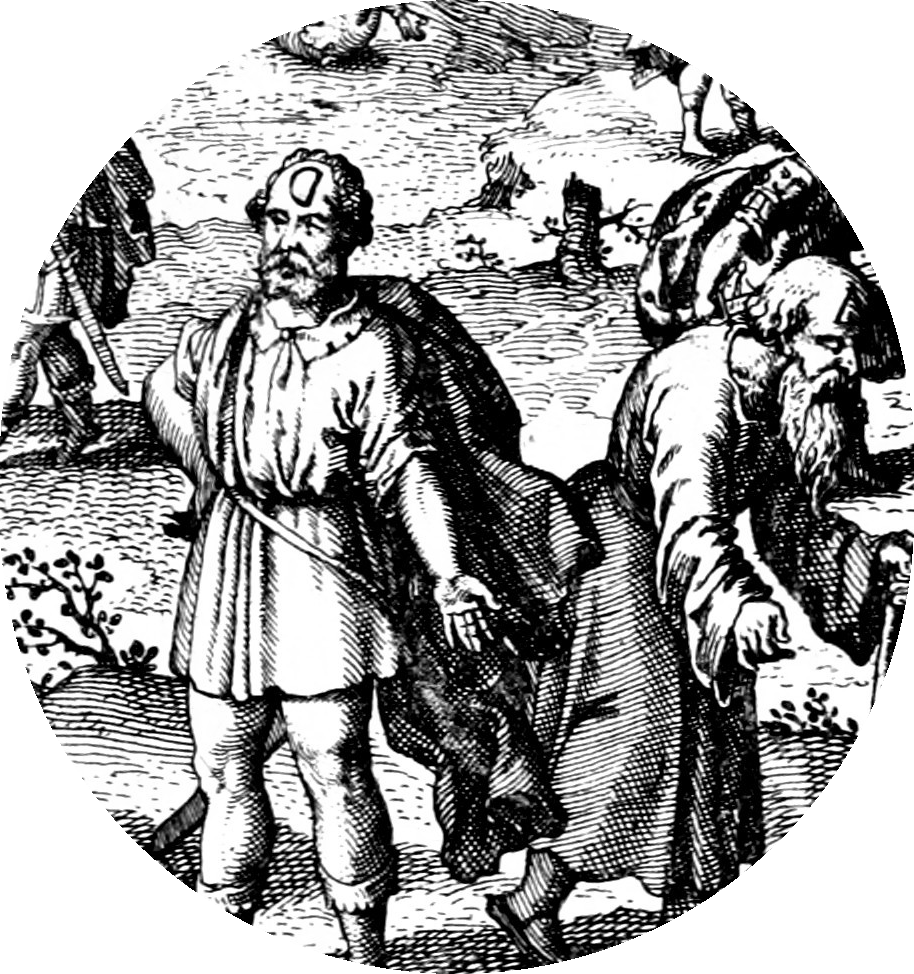
\includegraphics[width=0.6\textwidth]{images/brev19.png}
\end{center}

\breakpage